\section* {AIII.2}
\label {a3-2}
\subsection*{(i)}

Let $d$ denote the distance between 2 arbitrary vertices corresponding to $P$ and $d^*$ denote the distance after rounding $p_{i,x}, p_{i,y}$
where $p_{i,x}$ and $p_{i,y}$ denote the x- and y-coordinate of $p_i \in P$, by $\Delta$.

% euclidean distance equation
\begin{align*}
    d &= \sqrt[]{(p_{i,x} - p_{j,x})^2+ (p_{i,y} - p_{j,y})^2}   \\
    d^* &= \sqrt[]{(p_{i,x^*} - p_{j,x^*})^2+ (p_{i,y^*} - p_{j,y^*})^2}
\end{align*}

We know that the range of $p_x^*$  is

% range of p*
\begin{align*}
    \frac{px}{\Delta} \leq p^*_x \leq \frac{px}{\Delta} + 1
\end{align*}

Then we derive the range of $d^*$
\begin{align*}
    \sqrt[]{( \frac{p_{i,x}}{\Delta} - (\frac{p_{j,x}}{\Delta} + 1 ))^2+ (\frac{p_{i,y}}{\Delta} - (\frac{p_{j,y}}{\Delta}+1)^2}
    \leq d^* &\leq \, \sqrt[]{( \frac{p_{i,x}}{\Delta} + 1 - \frac{p_{j,x}}{\Delta})^2+ (\frac{p_{i,y}}{\Delta} + 1 - \frac{p_{j,y}}{\Delta})^2}   \\
\end{align*}

From the triangle inequality property, such that a, b and c are the lengh of the triangle edges
\begin{align*}
    c &\leq a + b
\end{align*}

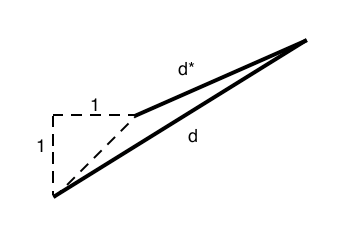
\includegraphics[scale=0.5]{3-2-lowerbound-d-star}
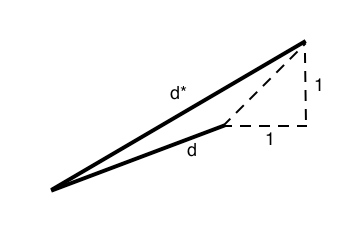
\includegraphics[scale=0.5]{3-2-upperbound-d-star}

We can simplify the range of $d^*$ to

\begin{align*}
    \sqrt[]{( \frac{p_{i,x}}{\Delta} - \frac{p_{j,x}}{\Delta})^2+ (\frac{p_{i,y}}{\Delta} - \frac{p_{j,y}}{\Delta})^2}
     - \sqrt[]{2}
    \leq d^* &\leq \, 
    \sqrt[]{( \frac{p_{i,x}}{\Delta} - \frac{p_{j,x}}{\Delta})^2+ (\frac{p_{i,y}}{\Delta} - \frac{p_{j,y}}{\Delta})^2}
     + \sqrt[]{2} \\
 \frac{d}{\Delta} - \sqrt[]{2} \leq d^* &\leq \frac{d}{\Delta} + \sqrt[]{2}
\end{align*}



% range of d*

Hence, the error of $d^*$  is $2\,\sqrt[]{2}$ at most.

The rounded integers are indeed the multiple of $\Delta$. Thus the maximum error of a single length is $2\Delta\sqrt{2}$. \\

Here we have $n$ lengths in the path. Therefore, the total error is:

% derive delta
\begin{align*}
    2n\,\sqrt[]{2}\Delta &= \varepsilon OPT\\
    \Delta &= \frac{\varepsilon OPT}{2n\,\sqrt[]{2}}\\
\end{align*}

\subsection*{(ii)}

Let $P$ and $P^*$ denote set of edges from the optimal solution and the PTAS algorithm respectively and we know that $length^*(P) \geq length^*(P^*)$, then we have
\begin{align*}
	\sum_{p_{i},p_{j} \in P^*}{d^*_{ij}} \leq \sum_{p_{i},p_{j} \in P}{d^*_{ij}}
\end{align*}

Thus, we can derive

\begin{align*}
	length(P^*) &= \sum_{p_{i},p_{j} \in P^*}{d_{ij}} \\
	&\leq \sum_{p_{i},p_{j} \in  P^*}{\Delta(d^*_{ij}+\sqrt[]{2})}  \\
	&\leq \Delta \sum_{p_{i},p_{j} \in  P^*}{(d^*_{ij}+\sqrt[]{2})} \\
	&\leq \Delta ( \sum_{p_{i},p_{j} \in  P^*}{d^*_{ij}}+|P^*|\,\sqrt[]{2}) \\
    &\leq \Delta ( \sum_{p_{i},p_{j} \in  P}{d^*_{ij}+|P^*|\,\sqrt[]{2})} \\
    &\leq \Delta ( \sum_{p_{i},p_{j} \in  P}{( \frac{ d_{ij} }{ \Delta} + \sqrt{2} } ) + n\,\sqrt{2} ) \\
    &\leq \Delta ( \sum_{p_{i},p_{j} \in  P}{\frac{d_{ij}}{\Delta}+2n\,\sqrt[]{2})} \\
    &\leq \sum_{p_{i},p_{j} \in  P}{d_{ij}} + \Delta 2 n \,\sqrt[]{2} \\
    &\leq length\left(P\right) + \Delta2n\,\sqrt[]{2} \\
    &\leq OPT + \left( \frac{\varepsilon OPT}{2n\,\sqrt[]{2}} \right) 2n\,\sqrt[]{2} \\
    &\leq (1 + \epsilon )OPT
\end{align*}


\subsection*{(iii)}

Let $m^*$ denote the new boundary of the coordinate after rounding $p_{x}, p_{y}$ to $p^*_{x}, p^*_{y}$
and we also know that
\begin{align*}
			m &= max(p_x,p_y ) \\
			OPT &\geq 2m
\end{align*}
Thus
\begin{align*}
			\frac{m}{\Delta} \leq m^* \leq \frac{m}{\Delta} + 1
\end{align*}

Then, we can derive the running time
\begin{align*}
	m* &\leq \frac{m}{\Delta} + 1 \\
	&\leq \frac{m2n\,\sqrt[]{2}}{\epsilon OPT}+1 \\
	&\leq \frac{m2n\,\sqrt[]{2}}{\epsilon 2m}+1 \\
	&\leq \frac{n\,\sqrt[]{2}}{\epsilon}+1 \\
\end{align*}

Therefore, the running time is
\begin{align*}
	O\left(nm^*\right) &= O\Big(n\frac{n\,\sqrt[]{2}}{\epsilon}+n \Big) \\
	&= O\Big(\frac{n^2\,\sqrt[]{2}}{\epsilon} \Big)
\end{align*}
